%!TEX root = ../cursus_fys6.tex

\chapter{De beginselen van Newton}
\label{debeginselenvannewton}

Het onderdeel binnen de mechanica dat zich met het verklarende principe bezighoudt, is de dynamica. Tot nu toe hebben we in de kinematica enkel bewegingen beschreven. We willen die bewegingen nu ook fysisch verklaren. De drie beginselen van Newton vormen, samen met enkele krachten, de fundamenten waarop de klassieke mechanica is gebouwd. 

\newpage

\section{De wet van de traagheid}

Op 22 oktober 1895 gebeurde er in het eindstation Gare Montparnasse -- Parijs, een ongeluk. De treinbestuurder was door het station gereden en pas 30 meter voorbij het einde van het spoor tot stilstand gekomen.
\begin{figure}[h]
\begin{center}
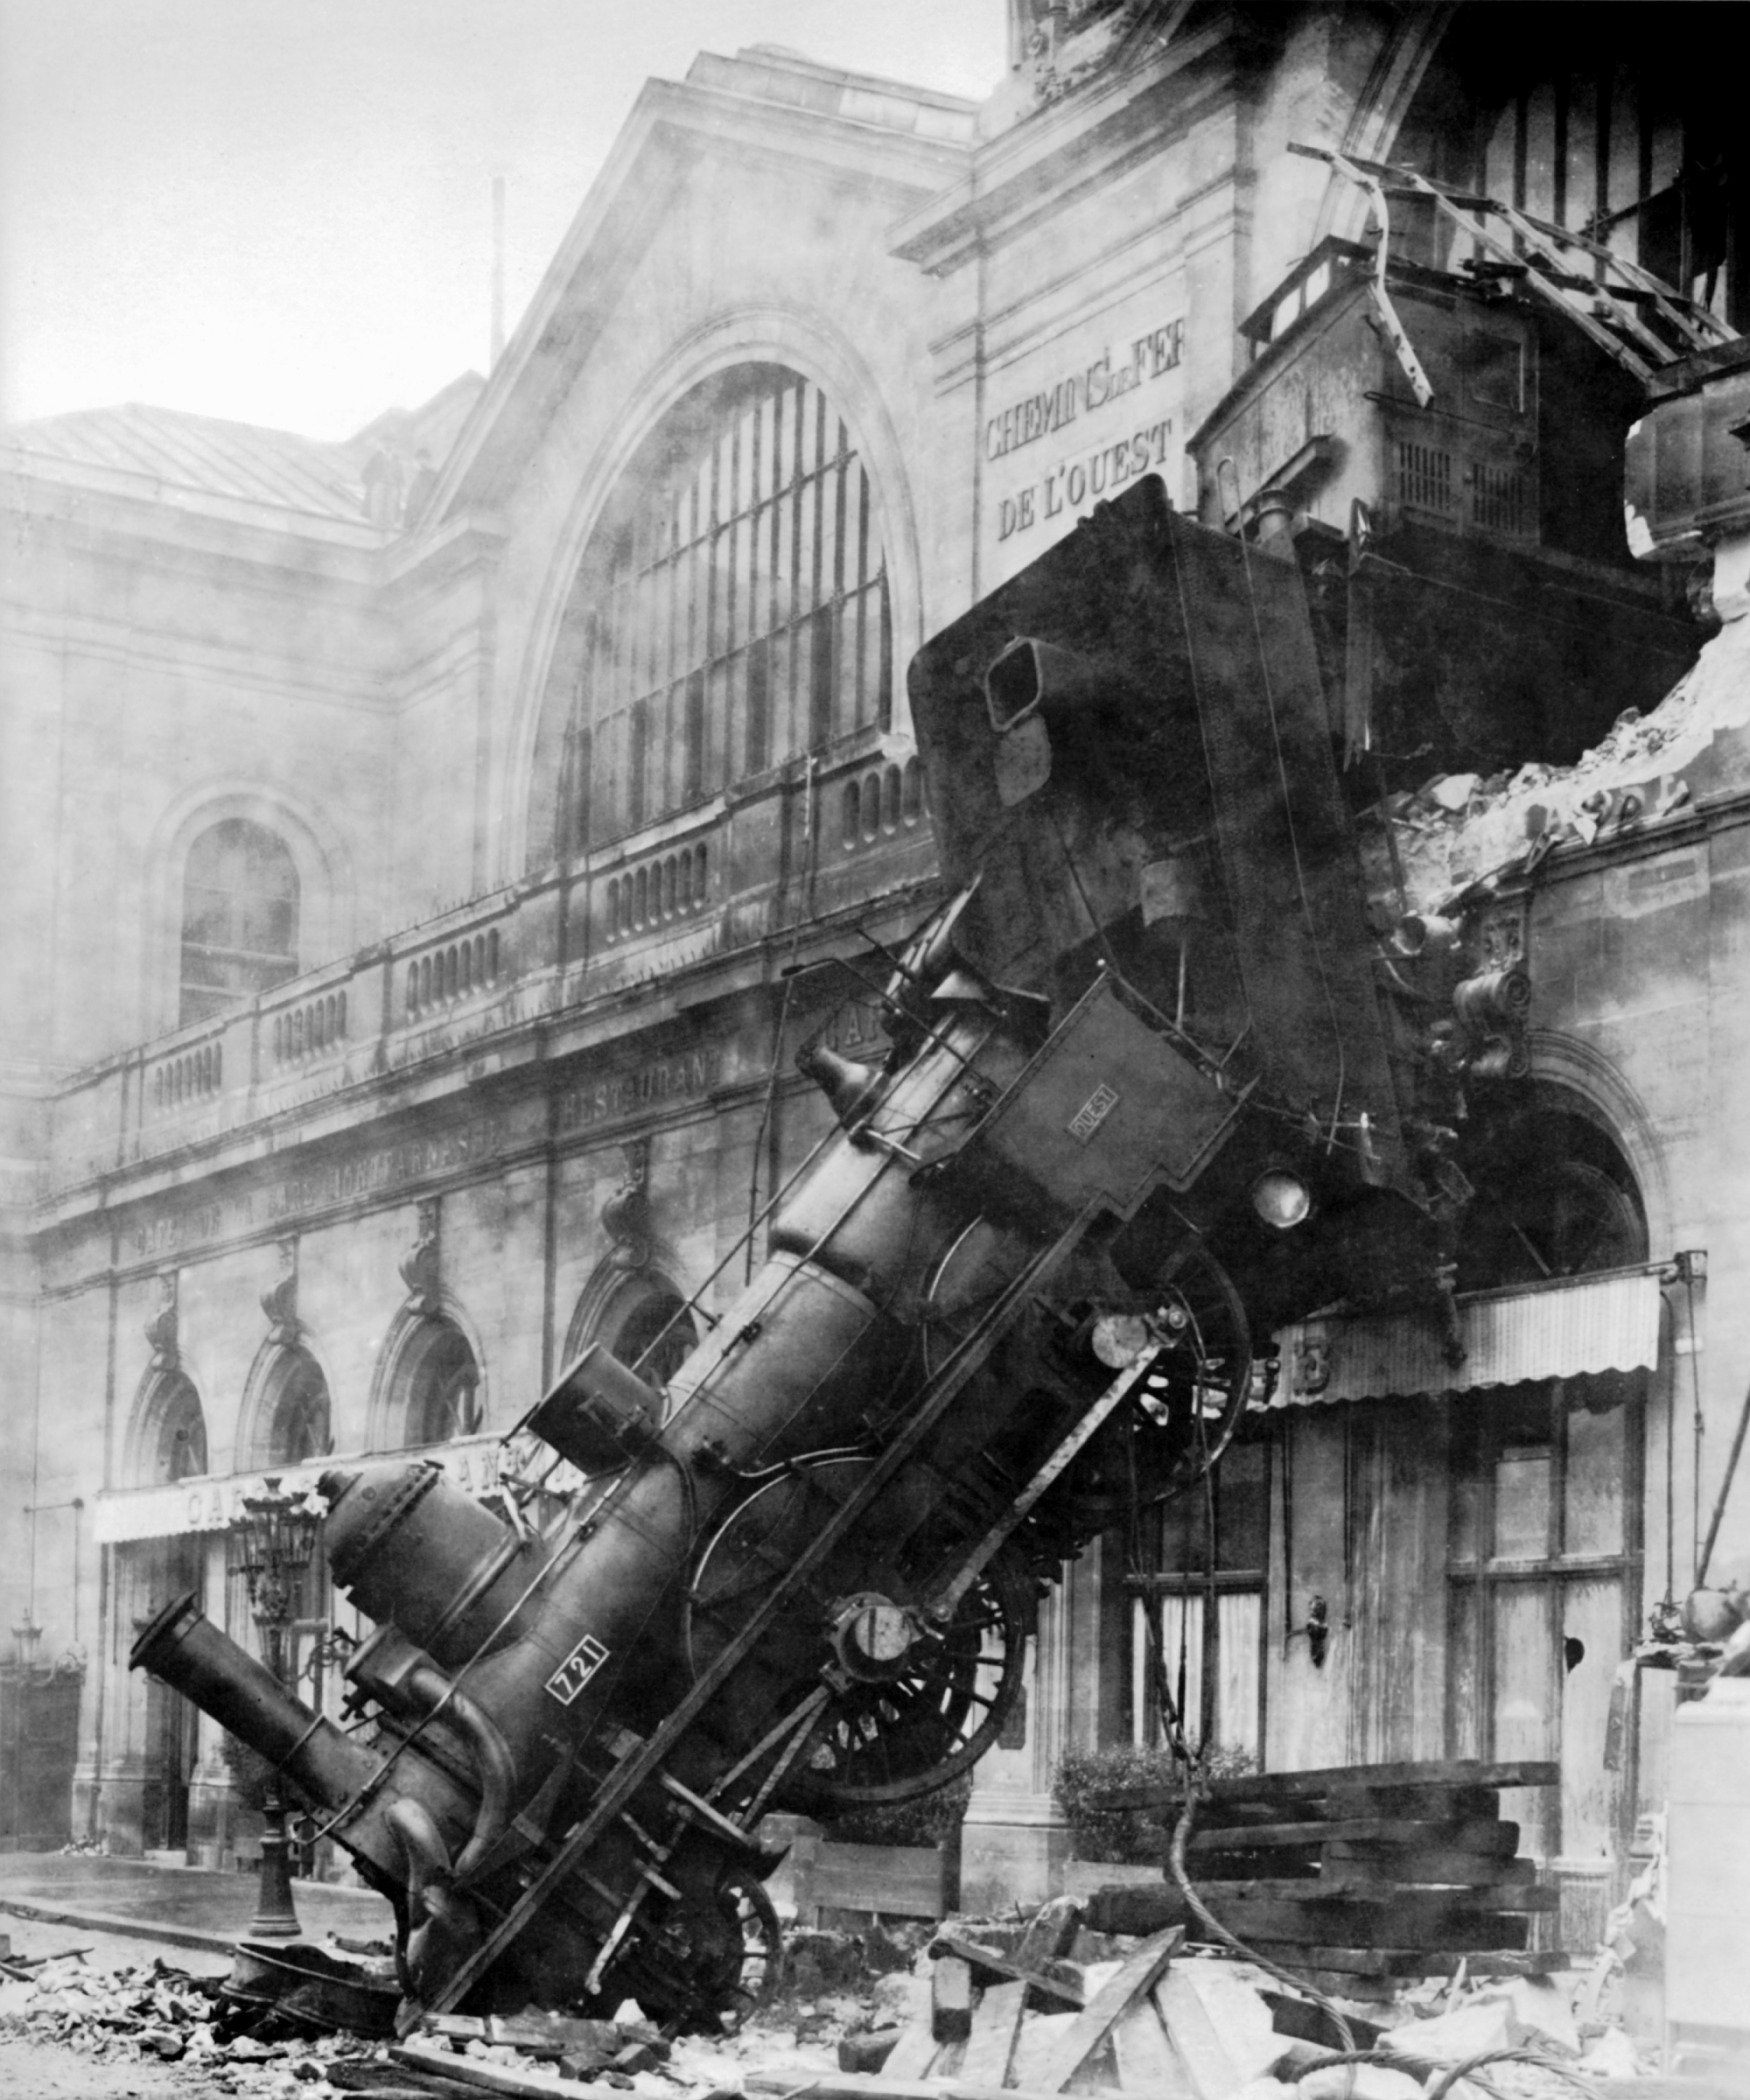
\includegraphics[width=.8\textwidth]{Train_wreck_at_Montparnasse_1895}
\caption{Gare Montparnasse. Parijs 1895}
\end{center}
\end{figure}

De figuur ademt de onvermijdelijke wet van de traagheid uit \ldots
\newline
\kader{
\vspace{1mm}
{\textbf{De wet van de traagheid}}

Een voorwerp behoudt zijn toestand van rust of van eenparige rechtlijnige beweging, tenzij er een resulterende kracht op werkt.
\vspace{3mm}}

Je zal zeggen dat je met die wet al vertrouwd bent. Maar zoals zo vaak, blijken we zonder het te beseffen niet zomaar alle consequenties in rekening te brengen. Onze ervaring uit het dagelijks leven
wil wel eens roet in het eten strooien. Zo zijn we vertrouwd met het feit dat
fietsen toch enige inspanning en dus kracht vergt. Zeker als de wind tegen zit.
We zouden dus kunnen aannemen dat -- willen we bewegen -- we steeds een kracht nodig
hebben en willen we harder bewegen, we een grotere kracht nodig hebben. Die kracht zou dan moeten dienen om om het streven naar de `natuurlijke' toestand van rust, tegen te gaan en de snelheid te onderhouden. Wat denk je, is dit niet in strijd met de wet van de traagheid \ldots?!\footnote{Als je tegen een topsnelheid van $300\rm\,km/h$ in de Thalys richting Parijs zit, voel je de zetel dan harder tegen jou duwen dan dat ze dat doet wanneer je nog stilstaat in Brussel-Zuid \ldots?}

Laten we -- om deze misvatting te bestrijden -- een gedachte-experiment uitvoeren. We doen dus niks concreets -- enkel redeneren. Het is een gedachte-experiment van Galileo Galilei (1564-1642). Om het uit te voeren hebben we een speciale knikkerbaan nodig, eentje zonder wrijving.\footnote{Ik heb horen zeggen dat er lang geleden een klein winkeltje bestond dat dergelijke knikkerbanen verkocht. Doorheen de jaren is het adres echter verloren gegaan. Niemand weet meer waar het zich bevindt \ldots} Laten we ervan uitgaan dat we in het bezit zijn van zo'n uiterst zeldzame baan. Onderstaande figuur toont dan de situatie waarin we een knikker op een bepaalde hoogte aan de linkerkant loslaten. Omdat er geen wrijving is, zal -- omwille van behoud van energie -- de knikker op de andere helling tot eenzelfde hoogte rollen, daar momentaan stilvallen en vervolgens terugrollen.
\begin{figure}[h]
\centering
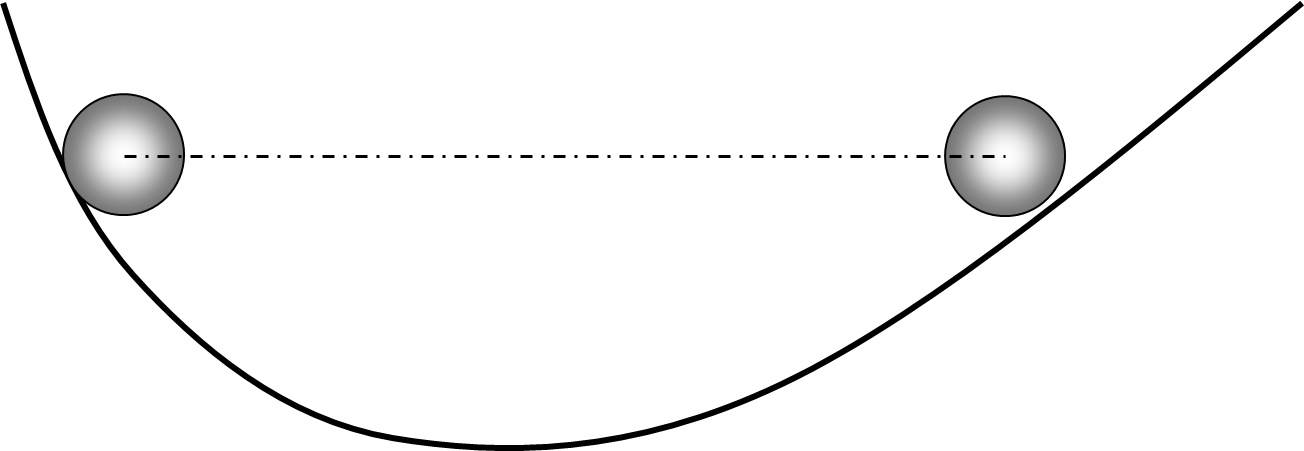
\includegraphics[width=.7\textwidth]{Afbeelding1}
%\caption{Het knikkertje rolt tot op dezelfde hoogte}
\label{Afbeelding1}
\end{figure}

Als we vervolgens de rechterhelling vlakker maken, zoals in onderstaande figuur, zal ons knikkertje ook nu tot dezelfde hoogte rollen. En dit ongeacht de grotere afstand. De energie-inhoud moet immers gelijk blijven.
\begin{figure}[h]
\centering
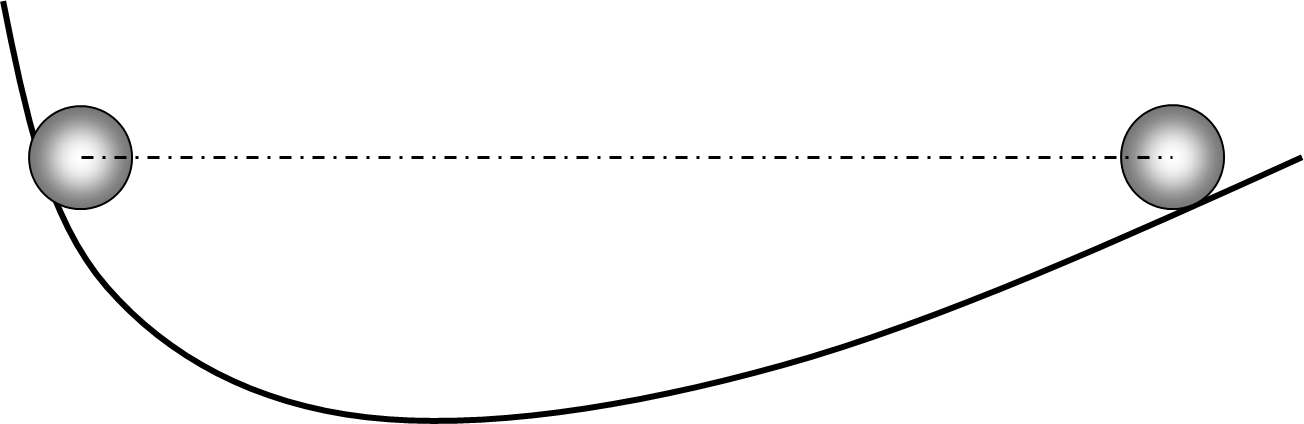
\includegraphics[width=.7\textwidth]{Afbeelding2}
\end{figure}

Als laatste stap in onze redenering, misleiden we ons knikkertje\footnote{Mag dat wel?}. Het knikkertje moet -- zo hebben we het hem verteld -- een tijdje horizontaal rollen om pas dan de rechterhelling te kunnen oprollen. Opnieuw tot dezelfde hoogte. Nu hebben we echter de rechterhelling oneindig ver weg gezet! Ons arm knikkertje zal dus blijven rollen (herinner u, er was geen wrijving) in de veronderstelling de helling ooit te zullen tegenkomen. 
\begin{figure}[h]
\centering
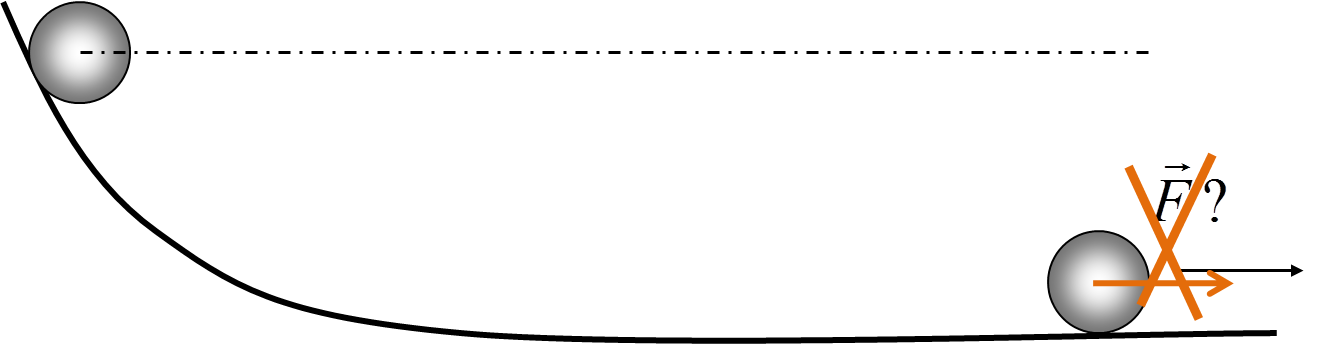
\includegraphics[width=.7\textwidth]{Afbeelding3}
\end{figure}
Gedurende het rollen op het horizontale stuk is de knikker dus niet onderhevig aan een voorwaartse kracht!\footnote{Wie zou immers die kracht uitoefenen \ldots?!} De beweging moet niet worden `onderhouden'. 

Uit ons gedachte-experiment kunnen we concluderen dat er een kracht nodig was om de knikker in beweging te brengen maar dat er \emph{geen} kracht nodig is om de beweging van de knikker op een rechte lijn en met een constante snelheid te onderhouden. Er is dus geen recht evenredig verband tussen kracht en snelheid \footnote{Moest je dat al denken.}. Kracht en snelheid kunnen zelfs tegengesteld zijn -- denk maar aan de wrijvingskracht die de beweging tegenwerkt.

De tendens van lichamen om zich te verzetten tegen de verandering van beweging, noemen we \textit{inertie} of \textit{traagheid}. Hoe groter de massa, hoe meer een voorwerp zich verzet.

\begin{figure}[h]
\centering
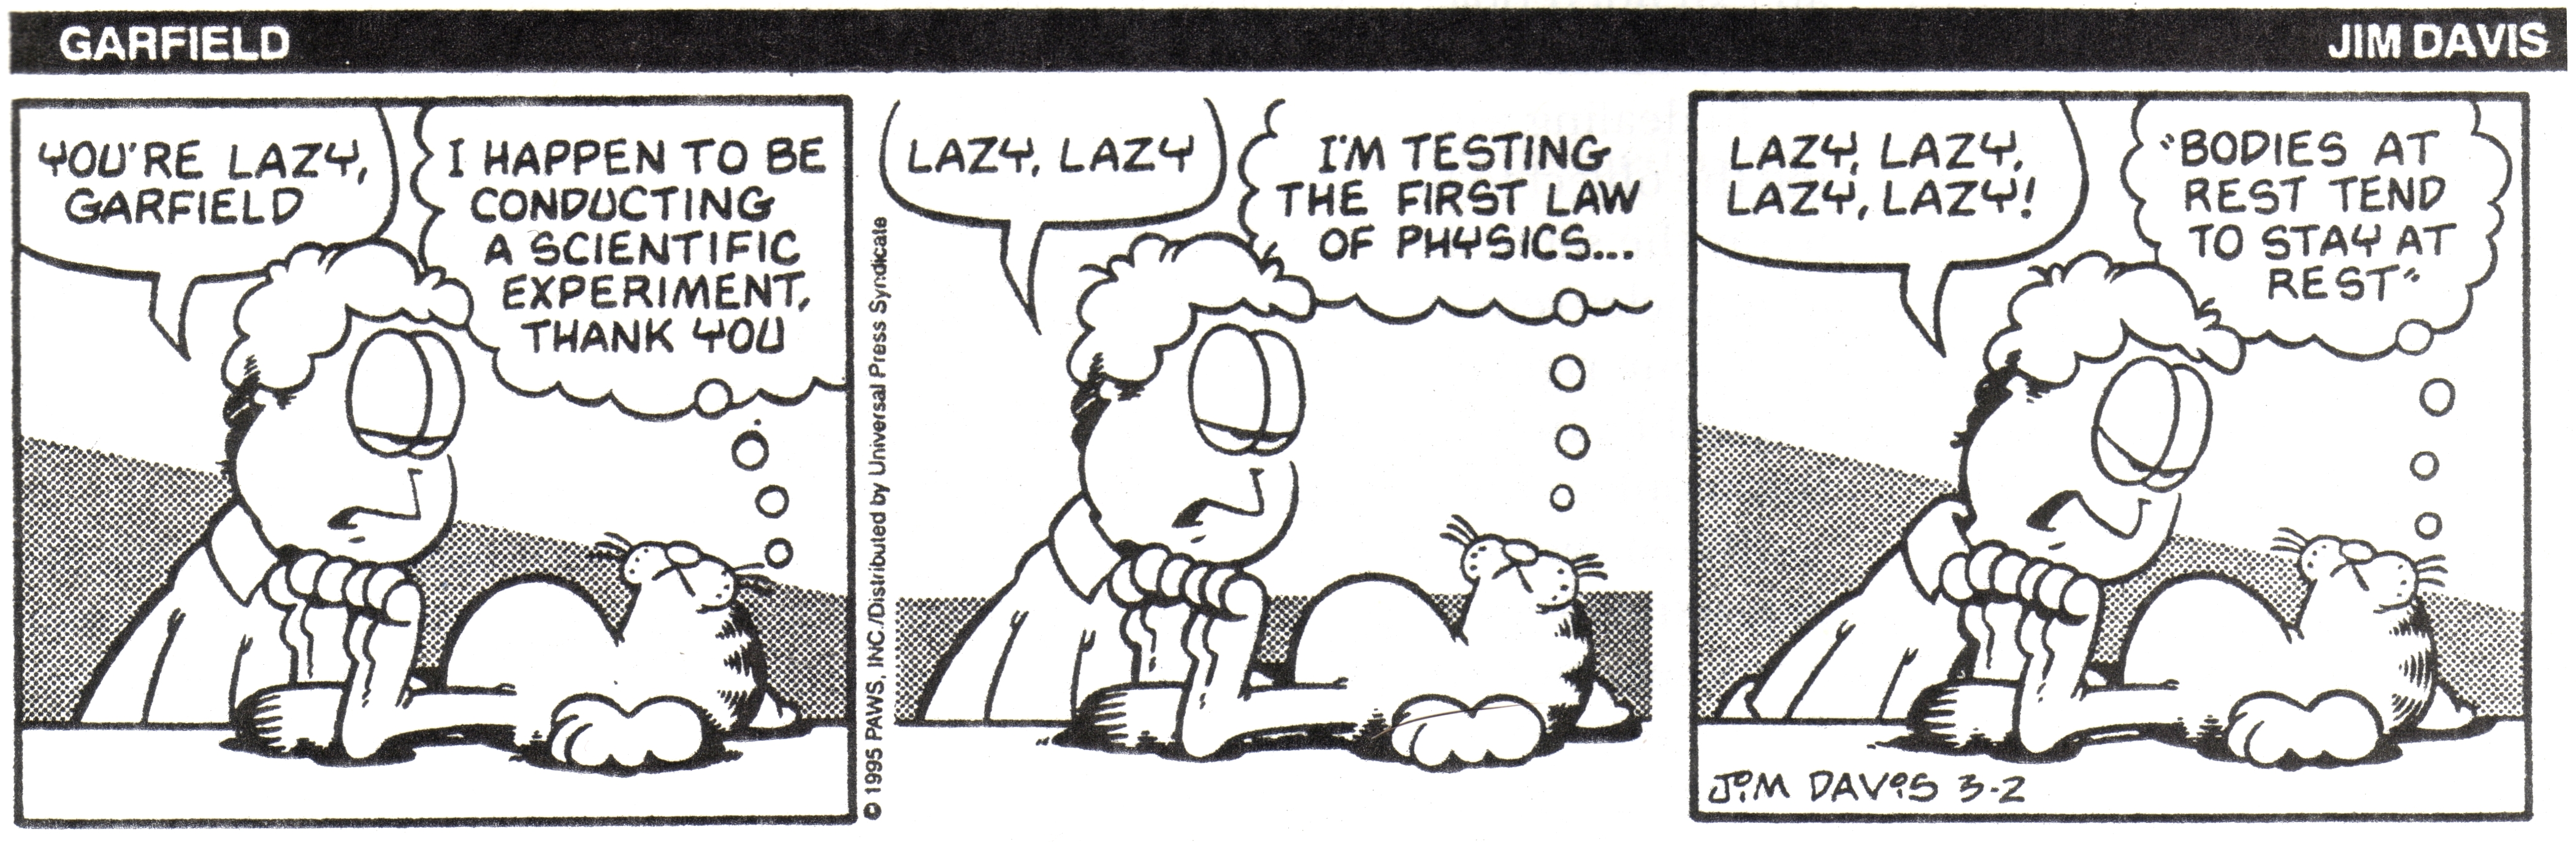
\includegraphics[width=0.8\textwidth]{Garfield_firstlaw}
\end{figure}

\voorbeeld{}{\textsf{
Wanneer je met de fiets fietst, rechtdoor en met een constante snelheid, is de kracht die je voorwaarts uitoefent dan groter, kleiner of gelijk aan de weerstandskracht die achterwaarts is gericht? Is met andere woorden de resulterende kracht op jouw fiets naar voren gericht, nul of naar achteren gericht? 
\newline
\newline Het antwoord is dat de resulterende kracht is nul is! Moest er immers een resulterende kracht zijn, dan zou volgens de wet van de traagheid de toestand van eenparige rechtlijnige beweging niet kunnen worden behouden. 
Eenmaal in beweging, is er geen kracht meer nodig om de beweging te onderhouden. Je moet blijven trappen om een even grote kracht als de weerstandskracht te kunnen genereren. Natuurlijk, om in beweging te komen, heb je wel een netto kracht naar voor toe nodig. Bij het remmen is de resulterende kracht dan weer naar achteren gericht.
}}

%\vfill


%\newpage

\section{Het tweede beginsel van Newton}

De eerste wet vertelt ons niet volledig wat er gebeurt wanneer op een lichaam een kracht werkt. Ze vertelt ons niet wat de relatie tussen kracht en beweging is. Uit onze dagelijkse ervaring zou je kunnen concluderen dat de snelheid van een voorwerp recht evenredig is met de erop uitgeoefende kracht. Hoe harder je immers op de pedalen duwt, hoe harder je gaat. De eerste wet vertelde ons echter al dat dit niet opgaat. 

Wat is dan de relatie tussen kracht en beweging? Een bal waar je harder tegen schopt, krijgt een grotere snelheid mee en een pingpongballetje vliegt gemakkelijker weg dan een basketbal of bowlingbal wanneer je er een tik tegen geeft. Als je het nader onderzoekt, door bijvoorbeeld verschillende krachten op een wagentje met eventueel steeds andere massa's te laten inwerken en de bijbehorende versnellingen te meten, merk je dat de versnelling recht evenredig is met de resulterende kracht en dat massa en versnelling omgekeerd evenredig zijn. M.a.w.
\begin{eqnarray*}
a\sim\frac{F}{m}
\end{eqnarray*}
%\begin{eqnarray*}
%\left.
%\begin{array}{l}
%\displaystyle
%a\sim F\\
%\displaystyle
%a\sim\frac{1}{m}
%\end{array}\right\}
%\Rightarrow a\sim\frac{F}{m}
%\end{eqnarray*}
Aangezien we met het fundament van de mechanica te maken hebben, kunnen we de eenheid van kracht zodanig kiezen dat de evenredigheidsconstante simpelweg 1 is. We defini\"eren dus \'e\'en newton als de kracht die een massa van \'e\'en kilogram een versnelling van \'e\'en meter per seconde kwadraat geeft. Samen met de observatie dat de versnelling dezelfde richting en zin als de kracht heeft, krijgen we de tweede wet van Newton.
\newline
\kader{
\vspace{3mm}
{\textbf{De tweede wet van Newton}}
\newline
\newline
De versnelling van een voorwerp is recht evenredig met de erop inwerkende resulterende kracht en omgekeerd evenredig met de massa van het voorwerp.
\begin{eqnarray*}
\vec{F}=m\vec{a}
\end{eqnarray*}
\vspace{0mm}}

Dit is misschien een gemakkelijke formule maar in al haar eenvoud \emph{immens} krachtig. Het is een wetmatigheid die een relatie geeft tussen de oorzaak (de krachten) en het gevolg (de beweging, strikt genomen de versnelling). Deze wetmatigheid is het verklarende principe achter alle mechanische bewegingen. Als we de krachten kennen, kennen we de versnelling van het voorwerp en kunnen we (althans op zijn minst in theorie) de baan van het voorwerp bepalen.


\section{Het derde beginsel van Newton}

Meestal plooien we onze vingers naar onze handpalm toe. De praktijk leert ons dat het andersom toch iets moeilijker gaat. Misschien vandaar. Als je echter met je andere hand wat helpt en duwt -- een kracht uitoefent -- plooien je vingers al iets verder naar achter. Uit zichzelf geraken ze niet zo ver. Als je nu -- ter vergelijking -- met gestrekte vingers tegen de tafel duwt, plooien je vingers eveneens meer naar achteren dan dat ze uit zichzelf zouden kunnen. Je moet concluderen dat naast het feit dat je een kracht op de tafel uitoefent\footnote{Misschien nu met weinig beweging tot gevolg.} de tafel op zijn beurt een kracht op je vingers uitoefent. Zonder extern inwerkende kracht zouden je vingers immers niet zo ver kunnen doorbuigen.
%\begin{figure}[h]
%\begin{center}
%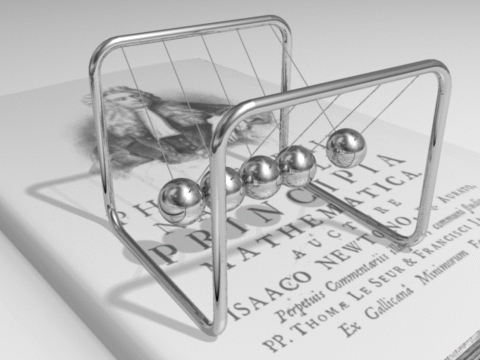
\includegraphics[width=.45\textwidth]{Newtons_cradle_animation_book}
%\caption{Een fascinerend speeltje}
%\end{center}
%\end{figure}
\begin{wrapfigure}{R}{0.5\textwidth}
\centering
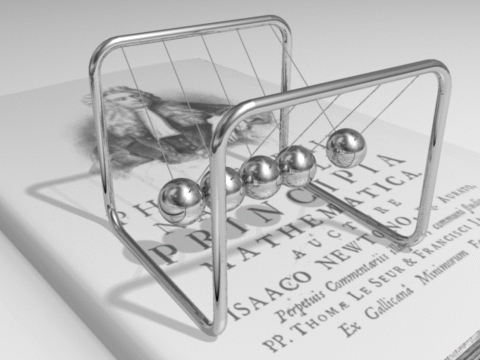
\includegraphics[width=0.44\textwidth]{Newtons_cradle_animation_book}
\caption{Een fascinerend speeltje}
\end{wrapfigure}
Een ander voorbeeld waarin lichamen krachten op mekaar uitoefenen is zo'n decoratief speeltje waar opgehangen metalen bolletjes op een fascinerende manier al botsend heen en weer slingeren. Een bolletje dat met een snelheid aangeslingerd komt, wordt tot stilstand gebracht terwijl een ander bolletje vanuit stilstand tot dezelfde snelheid wordt gelanceerd. Omdat de massa's van de kogeltjes even groot zijn en de versnelling van de ene even groot is als de vertraging van de andere, moeten de kogeltjes op elkaar even grote krachten uitoefenen. De derde wet van Newton -- ook wel de wet van actie en reactie genoemd -- \textit{poneert} dat de krachten die lichamen wederzijds uitoefenen \textit{altijd} even groot zijn.
\newline
\kader{
\vspace{1mm}
{\textbf{De wet van actie en reactie}}
\newline
\newline
Wanneer lichaam A op lichaam B een kracht uitoefent, oefent lichaam B op lichaam A een even grote maar tegengestelde kracht uit.
\begin{eqnarray*}
\vec{F}_{a,b}=-\vec{F}_{b,a}
\end{eqnarray*}
\vspace{0mm}
}

Met deze derde wet kunnen we verschillende verschijnselen verklaren. Zo is de wet van actie en reactie van toepassing op wandelen. Wij kunnen vanuit rust in beweging komen door ons af te zetten. Wij oefenen een kracht op de grond uit waarbij deze laatste op zijn beurt een even grote en tegengestelde kracht op ons uitoefent. Zo krijgen wij een versnelling. Een vliegtuig met straalmotoren of een raket doen hetzelfde. Door het uitoefenen van een kracht op de naar achter uitgeworpen gassen, oefenen de uitgeworpen gassen een kracht uit op het vliegtuig of de raket. Maar dan voorwaarts. (Een vliegtuig of raket duwt zich dus niet af tegen de (eventuele) lucht.)

Het even groot zijn van die krachten is misschien opmerkelijk. Het is toch de appel die naar de aarde valt en niet andersom?! Of, als de kracht die de aarde op de appel uitoefent even groot is als die de appel op de aarde uitoefent, waarom gaan ze dan niet naar mekaar toe? Het antwoord is dat de \emph{uitwerking} van een kracht niet hetzelfde is als de kracht zelf. De massa van de aarde is gigantisch veel groter dan die van de appel zodat die, volgens de tweede wet van Newton, een veel kleinere versnelling krijgt. En het is de versnelling die we zien, niet de kracht.

\newpage

\section{Oplossingsstrategie}

Bij het oplossen van vraagstukken waarin de wetten van Newton worden gebruikt, kan een vast stramien of heuristiek gebruikt worden. Omdat elke opgave anders is, blijft creativiteit noodzakelijk.
\begin{enumerate}
\item Bepaal het systeem dat je wilt beschouwen. Kies een systeem (object, lichaam, massa, geheel van lichamen) waarvan je een onbekende kracht of versnelling wilt berekenen. Kies een samengesteld systeem als je hierover informatie hebt.
\item Maak het systeem vrij. Beschouw het systeem als een vrij lichaam waarop alle uitwendige krachten inwerken. Teken al deze krachten die op het systeem werken. Dus niet de krachten die het systeem op zijn omgeving uitoefent. Die grijpen immers aan op een ander object. Het systeem waarop alle uitwendige krachten zijn getekend, wordt ook wel een krachtendiagram genoemd.
\item Pas de tweede wet van Newton toe op het systeem. Dit betekent dat de som van alle uitwendige krachten gelijk is aan de massa van het beschouwde systeem vermenigvuldigd met zijn versnelling:
\begin{eqnarray*}
\sum_{i=1}^n\vec{F}_i=m\vec{a}
\end{eqnarray*}
\item Kies een referentiestelsel en projecteer de vectorvergelijking. Ontbind de vectorvergelijking a.h.v. de eenheidsvectoren volgens de assen van een goed gekozen referentiestelsel. Op die manier bekom je
twee vergelijkingen die equivalent zijn met de vectorvergelijking:
\begin{eqnarray*}
x-as&:&\sum_{i=1}^nF_{i,x}=ma_x\\
y-as&:&\sum_{i=1}^nF_{i,y}=ma_y
\end{eqnarray*}
Hierin zijn $F_{i,x}$ en $F_{i,y}$ de componenten van de verschillende krachten volgens respectievelijk de $x$-as en de $y$-as.
\item Kies een tweede, derde \ldots systeem en herhaal stap 1 t/m 4. Indien er meer dan \'e\'en onbekende is, moet je nog andere systemen beschouwen. Kies ze zodanig dat je de derde wet van Newton kunt gebruiken tussen de verschillende systemen of dat de versnelling dezelfde is.
\item Los het stelsel vergelijkingen op.
\end{enumerate}

\newpage

\voorbeeld{}{\textsf{
\begin{enumerate}
\item[Opgave] Twee massa's $m_1$ en $m_2$ zijn via een touwtje en een katrol van te verwaarlozen massa met elkaar verbonden zoals in de figuur. Er is geen wrijving aanwezig. De massa's hebben een versnelling zoals aangegeven.
\newline
Bepaal de grootte van de versnelling van beide massa's en de grootte van de spankracht in het touw.
\begin{figure}[h]
\begin{center}
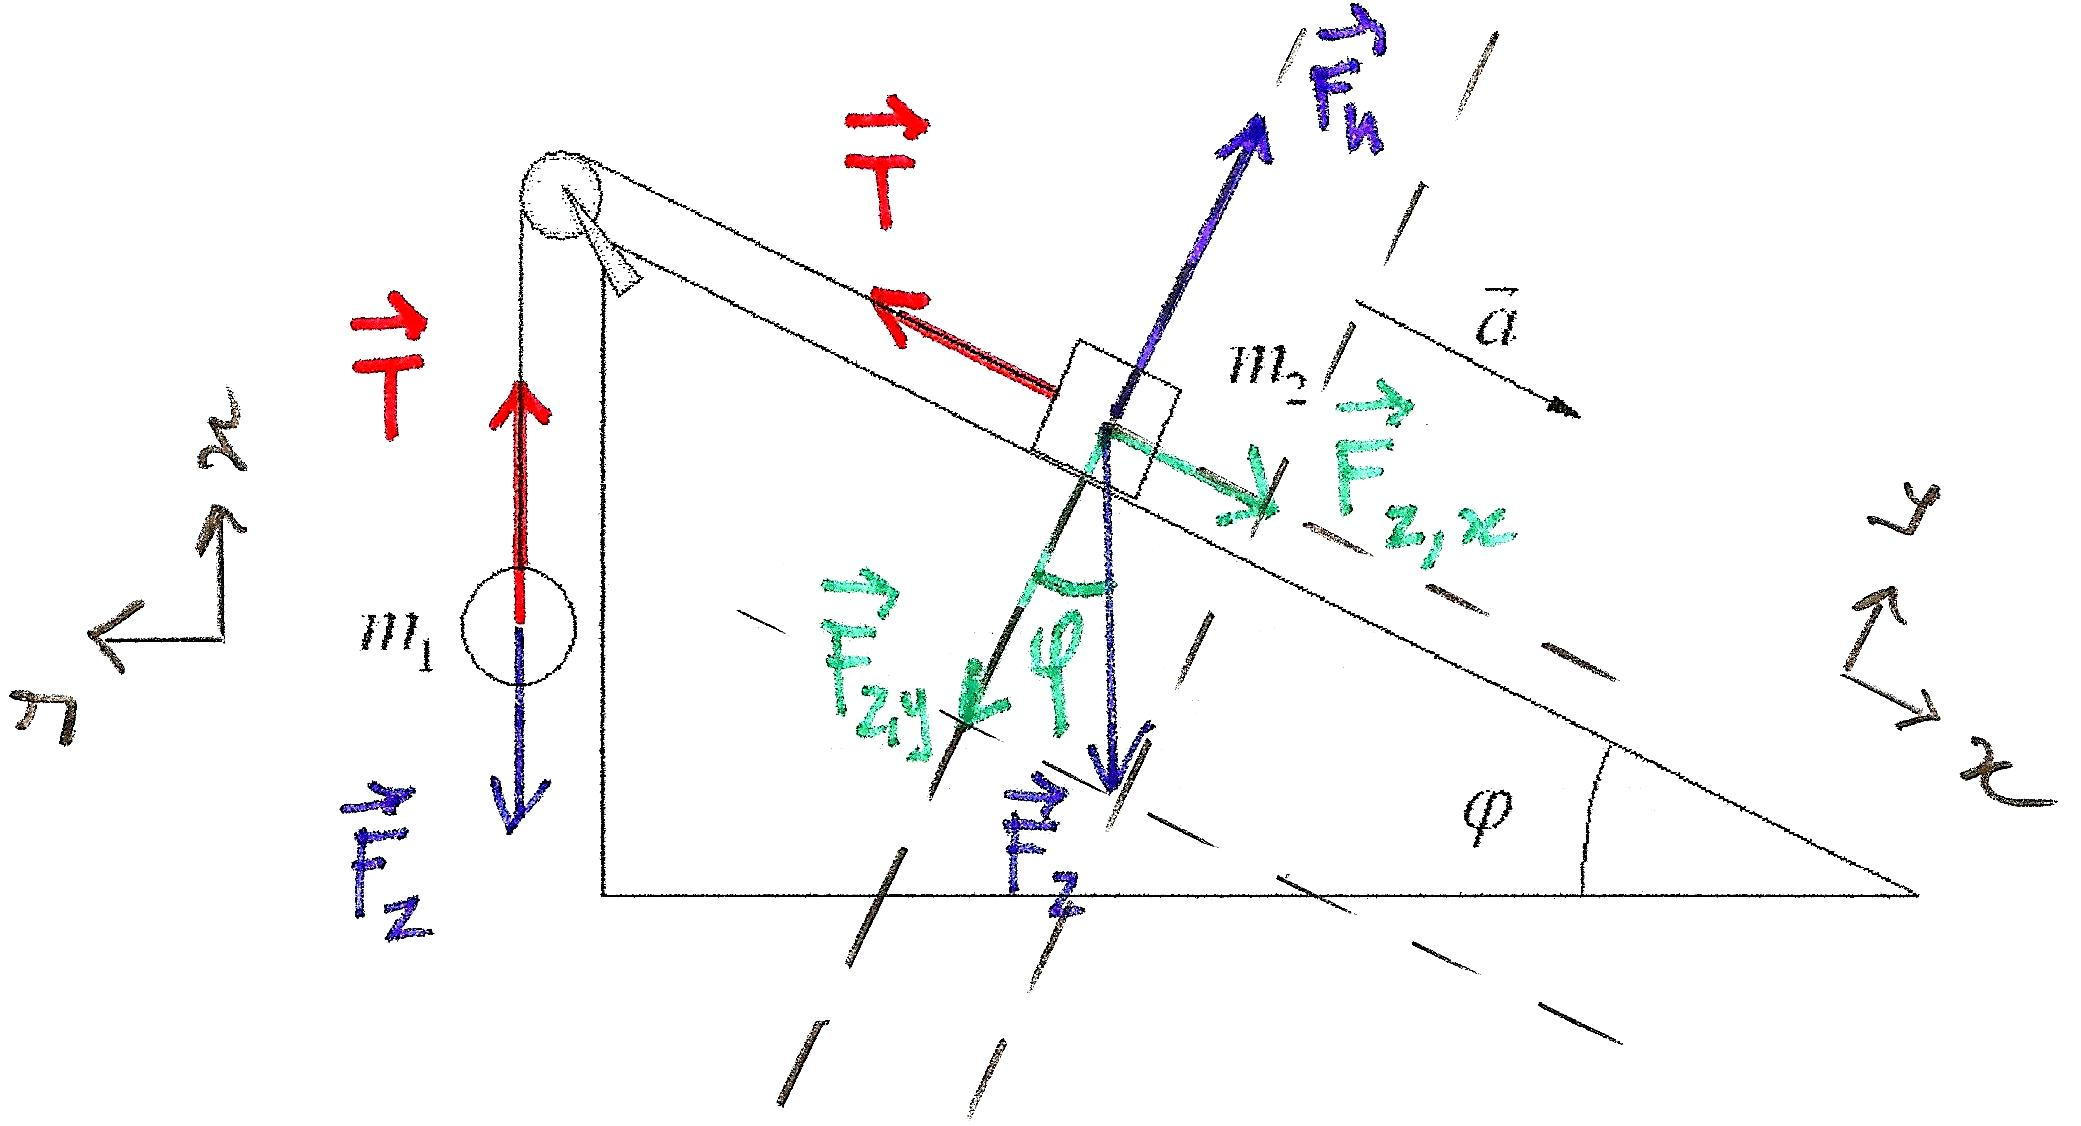
\includegraphics[width=0.45\textwidth, angle=0]{blokken_helling_opl}
\end{center}
\end{figure}
\item[gegeven]$m_1,~m_2,~\varphi$
\item [gevraagd]$a$, $F_s$
\item [oplossing]De tweede wet van Newton toepassen op $m_1$ levert
\begin{eqnarray}
F_s-m_1g&=&m_1a\nonumber\\
&\Updownarrow&\nonumber\\
F_s&=&m_1(a+g)\label{T1}
\end{eqnarray}
De tweede wet van Newton toepassen op $m_2$, met $F_z=mg$, levert
\begin{eqnarray}
F_{z,x}-F_s&=&m_2a\nonumber\\
&\Updownarrow&\nonumber\\
F_s&=&m_2(g\sin{\varphi}-a)\label{T2}
\end{eqnarray}
Uit (\ref{T1}) en (\ref{T2}) volgt
\begin{eqnarray}
%m_1(a+g)&=&m_2(g\sin{\varphi}-a)\nonumber\\
%&\Updownarrow&\nonumber\\
a&=&\frac{m_2\sin{\varphi}-m_1}{m_1+m_2}g\nonumber
\end{eqnarray}
Dit resultaat substitueren in (\ref{T2}) levert, na het uitwerken door op ge\-lij\-ke noemer te zetten:
\begin{eqnarray}
F_s&=&\frac{m_1m_2g(1+\sin{\varphi})}{m_1+m_2}\nonumber
\end{eqnarray}
\end{enumerate}
}}


\newpage


\section*{Dialogo sopra i due massimi sistemi del mondo}

Galileo schreef in 1632 een dialoog waarin hij de juistheid van het copernicaanse wereldbeeld fysisch probeerde te bewijzen door middel van de socratische methode\footnote{Van Dale: waarbij men de denkbeelden uit de geest van de leerling zelf ontwikkelt, terwijl men hem door gepaste vragen allengs zo ver brengt, dat hij het begrip, dat men hem duidelijk wil maken, zelf vindt.}. Een van de tegenargumenten was dat een vallende steen niet volgens een loodlijn op het aardoppervlak zou neerkomen, wanneer de aarde zelf een rotatie uitvoerde.\footnote{De aarde zou immers onder de steen wegdraaien.} Galileo haalde dit argument onderuit door gebruik te maken van het traagheidsbeginsel (anderen hadden dit ook geprobeerd via een 'slepende invloed' van de lucht, maar Galileo zag in dat dat niet voldoende was en erkent de ware fysische grondslag).
De dialoog gaat tussen drie geleerden. Sagredo is de vriend van een niet nader genoemd auteur (Galileo), die zijn gesprekspartners inlicht over diens nieuwe theori\"en. Salviati is de onbevooroordeelde geleerde die vooral zijn gezond verstand gebruikt, en dus de positie van de lezer verbeeldt. Simplicio is de wat simplistische schoolgeleerde (scholasticus), die het standpunt van Aristoteles weergeeft.
%\newline
%\newline
Hier een fragment uit deze dialoog.

\vfill

{\footnotesize

\begin{enumerate}
\item[SALVIATI]U zegt: aangezien bij een stilliggend schip een [vallende] steen aan de voet van de mast neerkomt, bij een bewegend schip daarentegen op enige afstand van de voet, kan men daaruit omgekeerd besluiten dat wanneer de steen aan de voet neervalt, het schip in rust is; en ook, dat wanneer het op enige afstand neerkomt, dat het schip dan beweegt. Aangezien datgene wat voor een schip geldt ook voor de hele Aarde moet gelden, volgt hieruit dat uit het neervallen van de steen aan de voet van de toren noodzakelijk tot de onbeweeglijkheid van de Aarde mag besloten worden. Is dat niet uw bewijs?
\item[SIMPLICIO]Ja, en op een zeer beknopte manier weergegeven, wat erg bijdraagt tot het goede begrip ervan.
\item[SALVIATI]Zeg me nu: als een uit de top van de mast losgelaten steen ook bij een snel bewegend schip precies op die plaats neervalt, waar het ook bij een stilliggend schip zou neerkomen, welke waarde zouden dan deze valexperimenten hebben voor het bepalen van de beweging of rust van het schip?
\item[SIMPLICIO]Helemaal geen waarde. Net zoals men uit de hartslag niet kan besluiten of iemand slaapt of wakker is, aangezien de hartslag op gelijke wijze klopt bij slapenden of wakenden.
\item[SALVIATI]Zeer goed. Hebt u ooit het experiment met het schip uitgevoerd?
\item[SIMPLICIO]Dat heb ik niet gedaan, maar ik denk wel dat de auteurs die ik daarnet genoemd heb, het zeer zorgvuldig hebben gecontroleerd. Bovendien ligt de oorzaak van het onderscheid zo voor de hand, dat hier nauwelijks enige ruimte voor twijfel overblijft.
\item[SALVIATI]Dat bepaalde auteurs het experiment mogelijk vermelden, zonder het zelf te hebben uitgevoerd, daarvan bent u zelf het beste bewijs. Want zonder het experiment te hebben uitgevoerd, noemt u het zeker en vertrouwt u op het woord van anderen. Net zo hebben mogelijk -- nee wel zeker -- ook die auteurs gehandeld, namelijk zich op hun voorgangers beroepen, zonder dat men ooit op een getuigenis is gestoten van iemand die het experiment werkelijk had uitgevoerd. Want iedereen die het uitvoert, zal vinden dat precies het tegenovergestelde plaatsvindt van datgene wat men in de boeken leest. Men zal namelijk tot het inzicht komen, dat de steen steeds op dezelfde plaats van het schip neervalt, of dat nu in rust is of in beweging met een willekeurige snelheid. En vermits de Aarde en het schip dezelfde verschijnselen moeten vertonen, zo mag men uit de loodrechte val van de steen en de inslag aan de voet van de toren niets besluiten over de beweging of de rust van de Aarde.
\item[SIMPLICIO]Als u mij niet het experiment als leidraad had aangewezen, dan zou onze discussie nog niet zo snel afgelopen zijn. Want dit probleem lijkt mij voor de menselijke rede zo moeilijk toegankelijk dat niemand hierin met enige geloofwaardigheid licht kan zien. 
\item[SALVIATI]En toch wil ik precies dat beweren.
\item[SIMPLICIO]U heeft dus niet eens honderd, zelfs niet \'e\'en experiment uitgevoerd en toch bent u reeds zeker van het resultaat? Ik hou vast aan mijn ongeloof en mijn aanvankelijke overtuiging, namelijk dat de voornaamste auteurs die het experiment vermelden, het ook uitgevoerd hebben en met de door hen aangegeven resultaten.
\item[SALVIATI]Ik ben zonder experiment zeker dat het experiment z\'o zal gebeuren zoals ik zeg, want het kan niet anders. Ja, meer nog, ik beweer zelfs dat u ook weet dat het resultaat niet anders kan zijn, al meent u of doet u zich voor het niet te weten. Ik versta echter de techniek om met hersens om te gaan zo meesterlijk, dat ik u zelfs tegen uw zin zal doen bekennen. [ ... ]
\item[SIMPLICIO]Ik zal uw vragen beantwoorden naar best vermogen, want ik ben zeker dat ik niet in moeilijkheden zal komen. Want van dingen waarvan ik weet dat ze niet waar zijn, kan ik toch moeilijk enige kennis hebben, aangezien kennis enkel kan bestaan over ware en niet over onware dingen.
\item[SALVIATI]Ik wil niet dat u mij iets antwoordt waarvan u niet zeker bent. Zeg me dan: als u een vlak oppervlak neemt, zo glad als een spiegel en gemaakt van een hard materiaal zoals staal, dat niet horizontaal is, maar een beetje hellend, en u legt daarop een perfect ronde kogel uit een zware, zeer harde stof, bijvoorbeeld brons, wat zal volgens u deze kogel, volledig aan zichzelf overgelaten, doen ? Meent u niet, net als ik, dat hij gewoon ter plaatse zal blijven liggen?
\item[SIMPLICIO]En het vlak is hellend?
\item[SALVIATI]Inderdaad, die onderstelling heb ik gemaakt. 
\item[SIMPLICIO]Ik geloof helemaal niet dat hij blijft liggen; in tegendeel, ik ben heel zeker dat hij uit zichzelf naar beneden zal rollen.
\item[SALVIATI]Let wel wat u zegt, Signor Simplicio; ik ben er namelijk van overtuigd dat de kogel overal zal blijven liggen, waar u hem ook legt.
\item[SIMPLICIO]Als u zich op zulke opvattingen vertrouwt, dan sta ik er niet meer versteld van dat u tot valse resultaten komt.
\item[SALVIATI]U houdt het dus voor zeker dat de kogel vanzelf naar beneden zal rollen?
\item[SIMPLICIO]Wat een vraag!
\item[SALVIATI]En u betrouwt hierop, niet omdat ik het u geleerd zou hebben -- ik heb immers getracht u het tegendeel te laten beweren -- maar helemaal uit uzelf, door toedoen van gezond verstand?
\item[SIMPLICIO]Nu begrijp ik uw truukje; u hebt slechts zo gepraat om mij uit mijn schelp te lokken, zoals men zegt, niet omdat u zelf daar zo over dacht.
\item[SALVIATI]Inderdaad. Hoe lang en met welke snelheid zal nu die kogel naar beneden rollen? Let op dat ik het hier heb om een volkomen ronde kogel en een perfect glad oppervlak, zodat alle uitwendige en toevallige hindernissen worden uitgesloten. Zelfs vraag ik u ook abstractie te maken van de luchtweerstand en van alle andere weerstanden, voor zover die zouden aanwezig zijn.
\item[SIMPLICIO]Ik heb alles goed verstaan. Op uw vraag antwoord ik: de kogel zal oneindig lang blijven rollen, zo lang het hellend vlak doorloopt, en wel in een eenparig versnelde beweging. Want zoals de natuur van zware lichamen het voorschrijft: vires acquirunt eundo. Daarbij zal de snelheid des te groter zijn, naarmate de helling van het vlak groter is.
\item[SALVIATI]Als men nu echter wil dat de kogel op het zelfde vlak naar boven beweegt, zal hij dat in de werkelijkheid ook doen?
\item[SIMPLICIO]Niet uit zichzelf; wel als men hem met geweld naar boven schuift of stoot.
\item[SALVIATI]En als de kogel nu met een zekere impuls naar boven wordt gestoten, wat zal dan zijn beweging zijn?
\item[SIMPLICIO]De beweging zou steeds langzamer worden, omdat zij tegennatuurlijk is. Verder zal zij langer of korter duren afhankelijk van de kracht van de stoot of de grootte van de helling.
\item[SALVIATI]U hebt nu, zo lijkt mij, het gedrag van een bewegend lichaam op twee verschillende vlakken geschetst. Op het hellend vlak, zegt u, beweegt het zware lichaam zich spontaan naar beneden met een eenparig versnelde beweging en om hem daar in rust te houden, moet men een kracht aanwenden; bij een stijgende helling is daarentegen een kracht nodig om hem vooruit te drijven en ook om hem vast te houden. De meegegeven hoeveelheid beweging, zegt u verder, vermindert in dit geval voortdurend en verdwijnt tenslotte geheel. Verder stelt u nog dat in beide gevallen de helling van het vlak van belang is; namelijk dat enerzijds een grotere helling ook een grotere snelheid met zich mee brengt en anderzijds een bewegend lichaam op een stijgende helling des te langer blijft bewegen naarmate de helling minder steil is. Zeg me nu wat met het lichaam zou gebeuren op een horizontaal oppervlak, dat niet daalt en niet stijgt.
\item[SIMPLICIO]Hier moet ik toch even over het antwoord nadenken. Aangezien er geen neerwaartse helling is, is er ook geen natuurlijke neiging tot bewegen; aangezien er verder ook geen opwaartse helling is, kan er ook geen weerstand tegen de beweging aanwezig zijn. Het lichaam moet dan onverschillig blijven tussen de neiging tot bewegen en de weerstand tegen die beweging. Het moet dan, volgens mij, van nature uit in rust blijven. - Maar hoe vergeetachtig ben ik toch! Nog niet zo lang geleden heeft Signor Sagredo me reeds uitgelegd dat dit precies het geval moet zijn.
\item[SALVIATI]Dat is ook mijn mening, in de onderstelling dat men de kogel rustig neerlegt. Als men hem echter met een impuls in een bepaalde richting wegstoot, wat zal dan gebeuren?
\item[SIMPLICIO]Het lichaam zal dan in die richting bewegen.
\item[SALVIATI]Maar welke beweging, een eenparig versnelde beweging, zoals in het geval van een neerwaartse helling, of een eenparig vertraagde, zoals bij de opwaartse helling?
\item[SIMPLICIO]Ik kan geen oorzaak voor een versnelling of een vertraging ontdekken, aangezien er geen neerwaartse of opwaartse helling is.
\item[SALVIATI]Goed. Als er echter geen oorzaak voor een vertraging is, dan zal er zeker geen oorzaak zijn om het lichaam geheel tot stilstand te brengen. Hoe ver zal het lichaam dan blijven bewegen?
\item[SIMPLICIO]Zolang de uitgebreidheid van het horizontale vlak het toelaat.
\item[SALVIATI]Als dit vlak onbegrensd zou zijn, dan zou de beweging van het lichaam evenzo onbegrensd zijn. Dus eeuwig?
\item[SIMPLICIO]Zo lijkt het me wel, tenminste als het lichaam van een bestendig materiaal is gemaakt.
\item[SALVIATI]Dat nemen we inderdaad aan, zoals we reeds gezegd hebben; alle toevallige en uitwendige hindernissen werden verwijderd en de vergankelijkheid van het voorwerp is ook zo'n toevallige hindernis. Zeg mij nu: wat is volgens u de reden waarom die kogel op een dalende helling spontaan, op een stijgende helling slechts dwangmatig beweegt?
\item[SIMPLICIO]De reden daarvan is dat de natuurlijke neiging van een zwaar lichaam erop gericht is zich naar het middelpunt van de aarde te bewegen, terwijl de opwaartse beweging naar de grenzen van het universum slechts met geweld kan plaats vinden. Het afhellend vlak maakt een nadering van het middelpunt mogelijk, het stijgende vlak echter de verwijdering.
\item[SALVIATI]Een vlak dat dus niet afhelt of stijgt, moet dus in al zijn delen even ver verwijderd zijn van het middelpunt. Bestaan dergelijke vlakken in de wereld?
\item[SIMPLICIO]Zo zijn er heel veel, bijvoorbeeld het aardoppervlak als het tenminste perfect glad zou zijn, en niet ruw en bergachtig, zoals het in werkelijkheid is. Maar neem bijvoorbeeld het wateroppervlak, zolang het water rustig en kalm is.
\item[SALVIATI]Een schip dat op een kalme zee vaart is dus zo een van de lichamen die zich voortbewegen op een horizontaal vlak, zoals we besproken hebben. Het zal dan ook, na wegnemen van alle toevallige en uitwendige hindernissen, voortdurend en onveranderd blijven voortbewegen met zijn eenmaal meegedeelde beginsnelheid.
\item[SIMPLICIO]Zo moet het zijn, lijkt me.
\item[SALVIATI]Nu, wat betreft de steen in de top van de mast. Beweegt die ook niet, gedragen door het schip, op een cirkelvormige baan rondom het middelpunt van de Aarde? Met andere woorden, heeft die steen geen beweging die, afgezien van uitwendige hindernissen, onuitwisbaar blijft voortbestaan? En is die beweging niet net zo snel als die van het schip?
\item[SIMPLICIO]Dat is allemaal juist. En dan?
\item[SALVIATI]Trek nu zelf het besluit uit het voorgaande, aangezien u alle premissen kent.
\item[SIMPLICIO]U bedoelt met het besluit, dat de steen, die beweegt met een onuitwisbare gedwongen beweging, deze beweging niet verliest [tijdens de val], maar het schip blijft volgen en tenslotte op dezelfde plek zal neerkomen als wanneer het schip stil ligt. En ik ook zeg dat dit het geval moet zijn als er geen uitwendige oorzaken zijn die de beweging van de losgelaten steen verstoren.
\end{enumerate}

}

\newpage

Het traagheidsbeginsel had bij Galilei nog geen universele status. Het ging slechts om een eigenschap van bewegingen van zware lichamen op een concentrische baan omheen het middelpunt van de aarde.
\newline
\newline
Hier een fragment uit Descartes' natuurkundeleerboek \textit{Principia Philoso\-phiae} (uitgegeven bij Elzevier te Leiden, 1644).
Descartes was een rationalist, d.w.z. dat hij de fundamentele natuurwetten baseerde op helder en `onbetwijfelbare' idee\"en in zijn geest, of bijvoorbeeld in de afwezigheid van redenen om iets anders aan te nemen. (`Waarom zou God ons misleiden door ons verkeerde idee\"en te laten denken?'). Descartes gaat iets verder dan Galilei, bij hem is het beginsel een algemene natuurwet, die niet enkel beperkt is tot zware voorwerpen onder invloed van de zwaartekracht, maar die inherent is aan het verschijnsel beweging.
\newline
\newline

{\footnotesize

\begin{enumerate}
\item[]\textit{De eerste wet der natuur: dat elk voorwerp blijft in die staat waarin het zich bevindt, zolang niets het verandert.}
Uit het feit dat ook God niet aan verandering onderhevig is, en dat Hij altijd op dezelfde wijze handelt, kunnen we kennis verwerven van bepaalde regels, die ik noem de wetten van de natuur, en die de oorzaken zijn van de verschillende bewegingen die we in alle lichamen waarnemen; belangrijk genoeg dus om hier te vermelden. De eerste is dat elk voorwerp voor zover mogelijk in dezelfde toestand blijft en die toestand slechts verandert door de interactie met andere. Zo zien we elke dag dat een vierkant voorwerp vierkant blijft, indien niets de vorm ervan wijzigt; en dat, als het voorwerp in rust is, het niet uit zichzelf begint te bewegen. Maar eenmaal het begonnen is te bewegen, hebben we ook geen enkele reden om te denken dat het ooit op eigen kracht zal ophouden te bewegen, zolang het niets ontmoet dat zijn beweging tegenhoudt of stopt. Zodat als een lichaam eenmaal begint te bewegen, wij moeten besluiten dat het steeds verder zal blijven bewegen, en dat het nooit uit zichzelf zal stoppen. Omdat we echter op een aarde leven die zodanig is opgebouwd dat alle bewegingen in onze omgeving vrij snel tot stilstand komen, en vaak door oorzaken die we met onze zintuigen niet kunnen waarnemen, oordelen we van jongs af aan dat de bewegingen die zo tot stilstand komen, dat uit zichzelf doen en hebben we nog steeds de neiging dat te geloven van alle bewegingen in de wereld, namelijk dat ze vanzelf tot stilstand komen en naar stilstand neigen, omdat we menen dat daarvan veelvuldige waarnemingen hebben gedaan. Nochtans is dat een verkeerd vooroordeel, dat duidelijk ingaat tegen de wetten van de natuur, want de rust is tegengesteld aan de beweging en niets zal door eigen instinct geneigd zijn tot zijn natuurlijk tegengestelde, of tot de vernietiging van zichzelf. [...]

\item[]\textit{De tweede wet van de natuur: dat elk bewegend lichaam zijn beweging zal trachten voort te
zetten volgens een rechte lijn.} De tweede wet die ik in de natuur opmerk, is dat elk deel van de materie op zich genomen nooit ernaar streeft zijn beweging verder te zetten volgens een gebogen baan, maar volgens een rechte lijn, hoewel vele lichamen kunnen gedwongen zijn af te buigen omdat ze andere lichamen op hun weg ontmoeten. [...] Deze wet, zoals de voorgaande, hangt af van het feit dat God onveranderlijk is, en dat hij de beweging van de materie behoudt door een eenvoudige handeling [namelijk van ogenblik tot ogenblik]. En hoewel de beweging zich niet voltrekt in een [ondeelbaar] ogenblik, toch is het duidelijk dat elk bewegend lichaam een richting aanhoudt volgens een rechte lijn en niet volgens een cirkelvormige. [...]

\item[]\textit{Waarin bestaat de kracht van een lichaam om te handelen of te weerstaan.} De kracht waarmee een lichaam inwerkt op een ander of de inwerking van dat andere lichaam weerstaat, ligt enkel hierin, dat elk ding voor zover mogelijk volhardt in de toestand waarin het zich bevindt, overeenkomstig de eerste wet. Zodat een lichaam dat verbonden is met een ander voorwerp een zekere kracht bezit om te verhinderen dat het ervan gescheiden wordt; en dat, wanneer het ervan gescheiden is, het een zekere kracht bezit om te verhinderen dat het ermee verbonden wordt. Ook, wanneer het in rust is, bezit het kracht om in rust te blijven en om te weerstaan aan alles wat het zou doen veranderen. Net als elk bewegend lichaam een kracht heeft om te blijven bewegen met dezelfde snelheid en in dezelfde richting. Men kan de grootte van deze kracht inschatten door de grootte van het voorwerp waarin ze huist, en van het oppervlak volgens hetwelk een voorwerp van een ander wordt gescheiden, en ook door de snelheid en de manier waarop botsende lichamen elkaar ontmoeten.

\end{enumerate}

}

De vruchtbaarheid van het traagheidsbeginsel komt pas goed tot uiting in het werk van Christiaan Huygens (1629-1695). Voor Huygens is het beginsel een algemeen aanvaard axioma waaruit de relativiteit van inerti\"ele stelsels kan afgeleid worden. Huygens ziet hierin een middel om de wetten van elastische botsing af te leiden, wat rond het midden van de zeventiende eeuw een nog helemaal onopgelost probleem
was. Descartes had met zijn traagheidsbeginsel een aantal botsingswetten geformuleerd die echter duidelijk fout waren, o.a. omdat de verschillende regels bij grensgevallen niet in elkaar overgingen. Huygens werkte op dit probleem vermoedelijk al in 1656, maar publiceerde pas in 1669 een kort verslag van zijn resultaten in de \textit{Philosophical Transactions} -- zonder enig bewijs. Pas na zijn dood werd het hele traktaat in zijn postuum \textit{Opuscula varia} (Leiden, 1703) openbaar gemaakt. Het geldt nog steeds als \'e\'en der mooiste teksten van de vroege fysica. De volgende tekst is de aanvang van het traktaat.
\newline
\newline
{\footnotesize

\begin{enumerate}
\item[Axioma 1] Een eenmaal bewogen lichaam zet, wanneer niets het belet, zijn beweging standvastig
voort met dezelfde snelheid en in rechte lijn.

\item[Axioma 2] Wat ook de oorzaak mag zijn van de botsing van twee harde lichamen, wij nemen de
volgende stelling aan: wanneer twee gelijke lichamen met gelijke snelheden uit tegenovergestelde
richtingen direct op elkaar stoten, wordt elk van beide met dezelfde snelheid als die waarmee het
aankwam, teruggeworpen. De botsing wordt direct genoemd, wanneer op dezelfde rechte die de
zwaartepunten verbindt, zowel de beweging als de botsing plaatsvindt.

\item[Axioma 3] De beweging van lichamen, de gelijkheid of ongelijkheid van snelheden, moet men
relatief opvatten, met betrekking op andere lichamen die men als in rust beschouwt, ook als deze
 misschien met andere een gemeenschappelijke beweging hebben. Wanneer dan twee lichamen op
 elkaar botsen, dragen zij op elkaar, ook als ze samen in nog een andere gemeenschappelijke,
eenparige beweging meegevoerd worden, slechts dezelfde impuls over als in het geval de
gemeenschappelijke beweging niet aanwezig was.
\newline
Zo stellen wij bijvoorbeeld dat wanneer iemand, die op een schip zit dat met een eenparige
snelheid vaart, twee gelijke kogels met gelijke snelheid op elkaar laat botsen -- let wel met
betrekking tot zichzelf en de delen van het schip -- dat beide ook met gelijke snelheid zullen
teruggestoten worden opnieuw met betrekking tot het schip, precies zoals wanneer het schip
stilligt of wanneer hij dezelfde kogels met gelijke snelheid liet botsen op het vasteland.
\end{enumerate}

}

\newpage

De tekst van Huygens werd zoals gezegd pas in 1703 bekend. In 1687 had Isaac Newton (1642-1727) intussen zijn `klassieke' formulering van de traagheidswet gegeven in \textit{Philosophiae Naturalis Principia Mathematica} (De wiskundige beginselen der natuurkunde, 1687). Maar is die formulering wel zo klassiek?
\newline
\newline
\textbf{Tekst 4}
{\footnotesize
\begin{enumerate}
\item[Definitie III] De \textit{vis insita} of inherente kracht van de materie, is het vermogen om te weerstaan, waardoor elk lichaam, voor zover het kan, zijn huidige toestand tracht te behouden, of het nu in rust is, of in uniforme, rechtlijnige beweging.
\newline
Deze kracht is steeds evenredig met het lichaam waartoe ze behoort en verschilt in niets van de
inactiviteit [inertie] van de massa, maar zoals wij die opvatten. Een lichaam zal omwille van de
inertie van de materie, niet gemakkelijk uit zijn rusttoestand worden gebracht. Daarom mag de \textit{vis
insita} ook zeer toepasselijk inertie- [\textit{vis inertiae}] of inactiviteitskracht worden genoemd. Maar een lichaam kan enkel deze kracht uitoefenen wanneer een andere kracht op het lichaam wordt uitgeoefend die tracht haar toestand te veranderen. De werking van de inertiekracht kan zowel weerstand als impuls worden genoemd; `weerstand' als het lichaam dat zijn toestand wil behouden, zich verzet tegen een uitwendige kracht; `impuls' wanneer het lichaam, door weerstand biedt aan de uitwendige kracht van een ander lichaam, tracht de toestand van het andere lichaam te veranderen. Weerstand wordt gewoonlijk gebruikt voor lichamen in rust en impuls voor lichamen in beweging; maar beweging en rust, zoals ze gewoonlijk worden opgevat, zijn slechts relatief onderscheiden. En evenmin zijn die lichamen die gewoonlijk als in rust worden beschouwd, ook werkelijk in rust. [...]

\item[Wet I] Elk lichaam blijft in de toestand van rust of gelijkvormige rechtlijnige beweging, tenzij het gedwongen wordt die toestand te veranderen door krachten die erop worden uitgeoefend.
\newline
Projectielen vervolgen hun beweging, in zover zij niet vertraagd worden door de weerstand van de lucht, of naar beneden gehaald worden door de zwaartekracht. Een tol, waarvan de delen door hun cohesie voortdurend van de rechtlijnige beweging worden afgebogen, zal zijn rotatie niet stopzetten, tenzij door de weerstand van de lucht. De grotere lichamen van planeten en kometen, die minder weerstand ontmoeten in vrije ruimtes, behouden hun bewegingen zowel rechtlijnig als cirkelvormig voor een veel langere tijd.

\end{enumerate}
}


\newpage

\textbf{Vragen}

\begin{enumerate}
\item Simplicio vertegenwoordigt in de tekst het standpunt van de scholastieke geleerden. Duid aan hoe Galilei hen portretteert.
\begin{oplossing}
\newline
Galilei portretteert hen als geleerden die de voor die tijd gangbare wetenschappelijke idee\"en aanhangen. 
\newline
Een van die idee\"en is het bewijs van het niet-roteren van de aarde. Omdat een steen aan de voet van een toren neervalt kan de aarde niet bewegen. Moest de aarde bewegen, dan zou immers tijdens het vallen de aarde onder de steen zijn verschoven en zou de steen op enige afstand van de toren terecht moeten komen. Galilei laat Simplicio deze misvatting bevestigen aan het begin van de dialoog waardoor Simplicio dus een scholastieke geleerde vertolkt.
\newline
Ook het niet uitvoeren van experimenten als toetssteen van wetenschappelijke theorie\"en is eigen aan de tijdsgeest op dat moment. Het louter menselijk redeneren en de autoriteit van voorgangers wordt als nodig en voldoende beschouwd om een ware kijk op de werkelijkheid te kunnen hebben. Galilei laat bovenaan pagina 34 Simplicio dit idee beamen wanneer Salviati het beschrijft.
\newline
Naast de twee hierboven genoemde misvattingen die de scholastieke geleerden volgens Galilei hebben, schetst hij hen wel als redelijke wezens. Zij beschikken over voldoende intellect om de eigenlijke waarheid wel te kennen. Anders zou hij immers niet via de socratische methode en dus ook het redeneren hen tot de juiste conclusie kunnen leiden. Aan het einde van de dialoog is het immers Simplicio die de juiste wetmatigheid (in de ogen van Galilei) geeft.
\end{oplossing}

\item Wat is de rol van het experiment bij Galilei?
\begin{oplossing}
\newline
Het experiment moet volgens Galilei dienen als rechter om te bepalen welke wetmatigheden de eigenlijke zijn. Simplicio zegt immers bovenaan pagina 34 dat zonder het experiment de eigenlijke uitkomst niet zomaar zal kunnen worden gevonden. Dit idee over de manier waarop aan wetenschap moet worden gedaan, is revolutionair in de wetenschappelijke evolutie. V\'o\'or Galilei stelde men zich namelijk nadat men zich via bepaalde argumenten had laten overtuigen, geen verdere vragen over de waarheid van idee\"en. 
\end{oplossing}

\item Waarin verschilt Galilei's traagheidsbegrip van het moderne?
\begin{oplossing}
\newline
Galilei's traageheidsbegrip verschilt in enkele opzichten van het moderne zoals we dat kennen onder de vorm van de eerste wet van Newton. Ten eerste is bij Galilei deze wetmatigheid gebonden aan de aardse context. Het op een rechte lijn bewegen is voor Galilei het bewegen op een cirkelvormige lijn die als middelpunt het middelpunt van de aarde heeft. Dit blijkt uit de zin die Salviati zegt op pagina 36: '\emph{Een vlak dat dus niet afhelt of stijgt, moet dus in al zijn delen even ver verwijderd zijn van het middelpunt.}' Ten tweede spreekt Galilei nog niet over het strakker omlijnde en abstracte begrip \emph{kracht} dat een beweging zal tegenwerken. Het gaat hier over \emph{toevallige en uitwendige hindernissen} zoals bijvoorbeeld een ruw oppervlak of vergankelijkheid. Als laatste heeft het traagheidsbegrip nog geen axiomatisch statuut bij Galilei. Voor Galilei is de traagheid een wetmatigheid van de natuur die zonder meer juist en waar is. Voor ons is het traagheidsbegrip een \emph{beginsel dat we aannemen als waar}. Het is een basis\emph{hypothese} die we waar veronderstellen voor zolang verschijnselen ermee overeenkomen en voor zolang ze niet wordt tegengesproken door waarnemingen.
\end{oplossing}

\item Galilei voert hier twee nieuwe analyse-technieken in: (1) redeneren vanuit een `ideaal' geval, dat in de werkelijkheid niet voorkomt; (2) de `continu\"iteit' van de natuurwetten, zodat men uit de studie van bekende verschijnselen iets kan afleiden van niet onderzochte gevallen. Duid deze twee technieken aan in Galilei's betoog.
\begin{oplossing}
\newline
De eerste analyse-techniek vinden we terug in de redeneringen over een kogel die volkomen rond is en een oppervlak dat perfect glad en oneindig lang is (p35 bovenaan). Zo worden immers de in de realiteit aanwezige hindernissen als niet-bestaande verondersteld.
\newline
De tweede analyse-techniek vinden we terug waar de conclusies van de redeneringen over de kogel en hellende vlakken worden toegepast op een vallende steen langs de mast van een schip (p36; '\emph{Nu, wat betreft de steen in de top van de mast. \ldots}') en vervolgens op een steen die van een toren valt (begin van de dialoog).
\end{oplossing}

\item Waarop steunt Descartes' bewijs van de wet van de traagheid. Waarin is het beter dan dat van
Galilei, waar is het minder goed?
\begin{oplossing}
\newline
De waarheid van de wetmatigheid steunt op het feit dat God niet aan verandering onderhevig is, dat Hij altijd op dezelfde manier handelt en dat (omdat God almachtig en goed is en ons dus juiste redeneringen moet kunnen laten maken) wij door helder te redeneren de wetmatigheden die God in de natuur heeft gelegd, kunnen vinden.
\newline
Bij Descartes gaat het niet langer over een cirkelvormige beweging maar over een rechtlijnige beweging. De wetmatigheid is zodoende niet meer verbonden met de aarde maar algemeen geldig. Hij beschouwt het ook als een wetmatigheid die de oorzaak is van de verschillende bewegingen. De wetmatigheid krijgt meer een verklarend principe. De toevoeging van het verzetten van lichamen tegen het samenkomen en van elkaar loskomen is minder goed omdat het een bijkomende wet suggereert.
\end{oplossing}

\item Hoe beoordeelt Descartes de zintuiglijke waarneming met betrekking tot zekere en ware
kennis?
\begin{oplossing}
\newline
Voor Descartes kunnen de zintuigen ons bedriegen. Doordat we immers verschillende keren hebben waargenomen dat voorwerpen tot stilstand komen, concluderen we valselijk dat voorwerpen dit uit zichzelf doen. Het is dus maar door zuiver te redeneren (en enkel door te redeneren) dat we tot de waarheid kunnen komen.
\end{oplossing}

\item Vergelijk de formulering van Huygens en Newton.

\item Wat is er van de \textit{vis insita} geworden in de huidige natuurkunde?

\item Vergelijk de voorbeelden die Galilei, Descartes, Huygens en Newton geven om het traagheidsbeginsel te onderbouwen. Welke zijn het beste gekozen?
\item Vergelijk de aanpak van Galilei, Descartes, Huygens en Newton.
\end{enumerate}

\clearpage
\newpage


